\section{Auswahl der Skriptsprachen}
\setauthor{Robert Freiseisen}

Die Wahl der Scriptsprachen wurde auf Grund von Internet-Recherchen 
und Fachgesprächen mit Mitschüler*innen und Professor*innen gefällt.\\
Folgende Scriptsprachen wurden gewählt:

\begin{itemize}
    \item Lua
    \item IronPython
    \item C\#script
    \item Javascript
\end{itemize}

\subsection{Lua}
Lua ist eine Programmiersprache, die für ihre hohe Ausführungsgeschwindigkeit geschätzt wird. 
Diese Schnelligkeit, kombiniert mit dem geringen Speicherbedarf der Sprache, macht sie ideal für ressourcenbeschränkte Umgebungen und eingebettete Systeme. 
Lua bietet eine "von Haus aus"-Nutzbarkeit, die es Entwicklern ermöglicht, sofort nach der Installation loszulegen, ohne sich um eine Vielzahl von Abhängigkeiten kümmern zu müssen. 
Ihre Einbettbarkeit ist ein weiteres Kernelement, das sie besonders attraktiv für Softwareprojekte macht, die eine integrierte Skriptsprache benötigen. Besonders in der Spieleindustrie hat Lua sich als beliebte Wahl für das Scripting etabliert. Hier ermöglicht es Entwicklern, schnell interaktive und flexible Spielmechanismen zu implementieren, ohne die Hauptspiellogik zu beeinträchtigen. 
Als Open-Source-Software steht Lua zudem einer breiten Entwicklergemeinschaft zur Verfügung, die zur kontinuierlichen Verbesserung und Erweiterung der Sprache beiträgt.
All diese Aspekte machen Lua zu einer vielseitigen Option für eine Reihe von Anwendungen, insbesondere für das Scripting in Videospielen, wie in "World of Warcraft" oder "Roblox".
\cite{gameScriptingMastery} \cite{luaDocs} \cite{programingInLua} \cite{nluaWebside} 

\newpage
\subsection{IronPython}
IronPython ist eine Open-Source-Implementierung der Programmiersprache Python, die auf der .NET-Plattform läuft. Es wurde ursprünglich von Jim Hugunin entwickelt und ist eng mit Microsoft assoziiert. IronPython ist in C\# geschrieben und ermöglicht die nahtlose Integration von Python-Code mit .NET-Anwendungen. Mit IronPython können Entwickler sowohl auf .NET-Bibliotheken als auch auf Python-Bibliotheken zugreifen, wodurch eine erweiterte Interoperabilität und Flexibilität erreicht wird.
IronPython unterstützt sowohl dynamische als auch statische Sprachfunktionen, und es ist durch die Common Language Runtime (CLR) von Microsoft vollständig integriert. Dies ermöglicht eine effiziente Ausführung von Python-Code auf der .NET-Plattform und erleichtert die Erstellung gemischter Anwendungen, die sowohl Python- als auch .NET-Code nutzen.
Beim Speicherverbrauch ist IronPython in der Regel nicht so effizient wie CPython, da das .NET mehr Overhead haben kann. 
Durch die Nutzung der Dynamic Language Runtime (DLR) von .NET kann IronPython dynamische Typen und späte Bindungen effizienter verwalten als einige andere Implementierungen, wie CPython. 
Dies ermöglicht eine enge Integration mit .NET-Bibliotheken und erleichtert die schnelle Entwicklung und Iteration von Code.
\cite{ironPython} \cite{ironPythonGithub} \cite{ironPythonInAction}
 
\newpage
\subsection{C\#script}
C\#Script ist ein Bestandteil der .NET-Plattform. Es ermöglicht die dynamische Ausführung von C\#-Code und ist in den .NET-Bibliotheken und -Laufzeitumgebungen enthalten. 
Einer der großen Vorteile von C\#Script ist, dass es sowohl in gehosteten als auch in eigenständigen Ausführungsmodellen eingesetzt werden kann. 
In einem gehosteten Modell kann das Skript innerhalb einer bestehenden Anwendung laufen und Objekte und Funktionen der Anwendung nutzen oder modifizieren. 
In einem eigenständigen Modell kann das Skript als unabhängige Anwendung ausgeführt werden. 
Ein weiteres wichtiges Merkmal ist die Kompatibilität mit .NET 5/Core und höheren Versionen. 
Dies ermöglicht eine bessere Leistung, erweiterte APIs und die Möglichkeit, plattformübergreifende Anwendungen zu entwickeln. 
Die Bibliothek stellt eine  Schnittstelle bereit, die die Integration von C\#-Skripten in eine Vielzahl von Anwendungsdomänen vereinfacht.

\cite{csharpScriptingArcticel}

\newpage 
\subsection{Javascript}
JavaScript ist eine populäre und vielseitige Programmiersprache, die vor allem in der Webentwicklung eingesetzt wird. 
Sie zeichnet sich durch ihre Einfachheit und Benutzerfreundlichkeit aus, was sie besonders für Einsteiger attraktiv macht. 
Die Sprache ist intuitiv aufgebaut, sodass die grundlegenden Konzepte schnell verstanden und angewendet werden können. 
Ein weiterer Vorteil ist, dass alle modernen Webbrowser eine JavaScript-Engine integriert haben. 
Dies ermöglicht es Entwicklern, Code unmittelbar im Browser auszuführen und zu testen, ohne zusätzliche Software installieren zu müssen. 
In Bezug auf die Sicherheit bietet JavaScript zwar einige Mechanismen, wie die Ausführung in einer Sandbox-Umgebung, um den Zugriff auf das Betriebssystem des Nutzers zu beschränken.  
Insgesamt bietet JavaScript eine ausgewogene Mischung aus Benutzerfreundlichkeit, Intuitivität und Funktionalität, allerdings müssen Entwickler stets wachsam in Bezug auf Sicherheitsrisiken sein.

Als .NET-Bibliothek wurde sich für "JavaScriptEngineSwitcher" mit "Jint" entschieden.
"JavaScriptEngineSwitcher" ist eine .NET-Bibliothek, die es ermöglicht, verschiedene JavaScript-Engines zu verwenden, und "Jint" ist eine JavaScript-Engine für .NET.


\cite{mDNWebDocs} \cite{owasp}

\newpage
\section{Kriterienkatalog}
\setauthor{Robert Freiseisen}
Jede der untersuchten Sprachen hat ihre eigenen Vor- und Nachteile, und die Auswahl der besten Option kann je nach Projektanforderungen variieren. 
In diesem Abschnitt betrachten wir diese vier Sprachen im Kontext von .NET unter verschiedenen Aspekten:

\begin{itemize}
    \item Aktivität der Entwicklung: 
    \begin{itemize}
        \item Wie lebendig und aktiv ist die Community hinter der Sprache? 
        \item Wie oft werden Updates veröffentlicht, und wie gut ist die Dokumentation?
    \end{itemize}
    \item Funktionalität:
    \begin{itemize}
        \item Welche Features bietet die Sprache, und wie reichhaltig ist ihr Ökosystem? 
        \item Gibt es umfangreiche Bibliotheken, die die Entwicklung erleichtern?
    \end{itemize}
    \item Einsetzbarkeit:
    \begin{itemize}
        \item Wie einfach lässt sich die Sprache in bestehende oder neue .NET-Projekte integrieren?
        \item Welche Voraussetzungen müssen erfüllt sein, und wie komplex ist die Integration?
    \end{itemize}
    \item Performance:
    \begin{itemize}
        \item Wie steht es um die Laufzeit-Performance des Codes? 
        \item  Inwiefern beeinflusst die Wahl der Sprache die Geschwindigkeit und Ressourceneffizienz der fertigen Anwendung?
    \end{itemize}
    \item Debugging:
    \begin{itemize}
        \item Welche Möglichkeiten bietet die Sprache für das Debugging von Code?
        \item Wie effektiv lassen sich Fehler finden und beheben, und welche Werkzeuge stehen zur Verfügung?
    \end{itemize}
\end{itemize}

\newpage
Alle Daten wurden auf zwei unterschiedlichen Geräten gemessen, da somit die Messungen gleichzeitig durchgeführt werden konnten.
Weil zwei verschiedene PCs für einen Vergleich genutzt wurden, kann dies die Vergleichbarkeit der Ergebnisse beeinflussen.

Folgende Gründe können dabei ein Faktor sein:

\begin{itemize}
    \item Hardware-Unterschiede: 
    \begin{itemize}
        \item Verschiedene PCs können erhebliche Hardware-Unterschiede aufweisen, darunter Prozessorgeschwindigkeit, Arbeitsspeicher, Grafikkarte, Festplattenkapazität und andere technische Spezifikationen. Diese Unterschiede können die Leistungsfähigkeit und Geschwindigkeit der beiden PCs stark beeinflussen.
    \end{itemize}
    \item  Betriebssystem und Software:
    \begin{itemize}
        \item Verschiedene PCs können unterschiedliche Betriebssysteme (z.B. Windows, macOS, Linux) und Softwarekonfigurationen aufweisen. Dies kann die Vergleichbarkeit der Ergebnisse beeinflussen, da bestimmte Anwendungen oder Aufgaben auf unterschiedlichen Betriebssystemen möglicherweise unterschiedlich ausgeführt werden.
    \end{itemize}
    \item Treiber und Updates:
    \begin{itemize}
        \item Die Installation und Aktualisierung von Treibern und Software kann zwischen verschiedenen PCs variieren. Dies kann zu unterschiedlichem Verhalten von Hardwarekomponenten und zur Auswirkung auf die Leistung führen.
    \end{itemize}
    \item Alter und Verschleiß:
    \begin{itemize}
        \item Ältere PCs könnten aufgrund von Abnutzung und Alterungsprozessen möglicherweise nicht mehr die gleiche Leistung erbringen wie neuere Modelle. Dies kann zu Unterschieden in der Vergleichbarkeit der Ergebnisse führen.
    \end{itemize}
    \item Systemkonfiguration: 
    \begin{itemize}
        \item Die Konfiguration von Betriebssystemeinstellungen, Energieeinstellungen und Hintergrundanwendungen kann zwischen den beiden PCs variieren, was sich auf die Ressourcennutzung und somit auf die Vergleichbarkeit auswirken kann.
    \end{itemize}
\end{itemize}

Die Daten für IronPython und Lua wurden auf den PC von Robert Freiseisen unter folgenden Voraussetzungen  gemessen:
\begin{itemize}
    \item Gerätspezifikationen:
    \begin{table}[H]
        \center
        \begin{tabular}{|p{3cm}|p{4cm}|}
            \hline
            Hersteller & HP \\ \hline
            Gerätname & LAPTOP-5U1879KR \\ \hline
            Prozessor & Intel(R) Core(TM) i5-8265U CPU @ 1.60GHz   1.80 GHz \\ \hline
            Installierter RAM & 8.00 GB (7.89 GB verwendbar) \\ \hline
            Produkt-ID & 00325-81357-65742-AAOEM \\ \hline
            Systemtyp & 64-Bit-Betriebssystem, x64-basierter Prozessor \\ \hline
        \end{tabular}
    \end{table}
    \item Betriebssystem:
    \begin{table}[H]
        \center
        \begin{tabular}{|p{4cm}|p{4cm}|}
            \hline
            Edition & Windows 11 Home \\ \hline
            Version & 21H2 \\ \hline
            Installiert am & 24.11.2021 \\ \hline
            Betriebssystembuild & 220.001.098 \\ \hline
            Leistung & Windows Feature Experience Pack 1000.22000.1098.0 \\ \hline
        \end{tabular}        
    \end{table}
\end{itemize}

\newpage
Die Daten für C\#script und Javascript wurden auf den PC von Philipp
PC B unter folgenden Voraussetzungen  gemessen:
\begin{itemize}
    \item Gerätspezifikationen:
    \begin{table}[H]
        \center
        \begin{tabular}{|p{3cm}|p{3cm}|}
            \hline
            Hersteller & Selber Gebaut \\ \hline
            Gerätname & PC-Philipp \\ \hline
            Prozessor & AMD Ryzen 5 1600 Six-Core Processor 3.20 GHz \\ \hline
            Installierter RAM & 16.00 GB \\ \hline
            Produkt-ID & 00330-80000-00000-AA542 \\ \hline
            Systemtyp & 64-Bit-Betriebssystem, x64-basierter Prozessor \\ \hline
        \end{tabular}
    \end{table}
    \item Betriebssystem:
    \begin{table}[H]
        \center
        \begin{tabular}{|p{4cm}|p{4cm}|}
            \hline
            Edition & Windows 10 Pro \\ \hline
            Version & 22H2 \\ \hline
            Installiert am & 17.08.2020 \\ \hline
            Betriebssystembuild & 19045.3393 \\ \hline
            Leistung & Windows Feature Experience Pack 1000.19044.1000.0 \\ \hline
        \end{tabular}        
    \end{table}
\end{itemize}


\newpage
\subsection{Aktivität der Entwicklung}

In der nachfolgenden Tabelle wird dargestellt, wie intensiv die Entwicklerteams an den unterschiedlichen Scriptsprachen arbeiten und ob diese auch die Nuget-Pakete entwickeln.
Es ist zu beachten, dass die Daten am 30.11.2022 erfasst wurden.
\begin{table}[H]
    \begin{tabular}{|p{3cm}|p{3cm}|p{3cm}|p{3cm}|p{3cm}|}
        \hline
        Aktivität & IronPython & Lua & C\#Scripting & Javascript\\ \hline
        Commits in den letzten 10 Monaten & 179 & 27 & 702 & 1153 \\ \hline
        Nuget-Packages vom Sprach-entwicklerteam selber &Nein &Nein &Ja & Nein\\ \hline
        Releases in den letzten 10 Monaten & 2 (2.7.1 und 3.4.0-beta1) & 1 (v5.4.4) & v4.0.0 und höher & v4.6.2 (und höher)\\ \hline
        Unterstützt aktuelle major Versionen von Scriptsprache & Ja & Ja & Ja & Ja\\ \hline
        Unterstützt aktuelle Versionen von .NET & Ja & Ja & Ja & Ja \\ \hline
    \end{tabular}
\end{table}

\subsection{Einsetzbarkeit}
Alle untersuchten Bibliotheken sind auf Windows, MAC und Linux lauffähig.

\newpage
\subsection{Performance}
Der Speicherplatz auf dem Laufwerk wurde aus dem Windows-File-Explorer entnommen. 
Die Geschwindigkeitsmessungen erfolgten mit BenchmarkDotNet. 
BenchmarkDotNet wird im Abschnitt \hyperref[sec:tech]{Verwendete Technologien} näher erleutert.

IronPython und NLua müssen externe Runtimes (für Python bzw. Lua) in die .NET-Umgebung integrieren, was zu zusätzlichem Overhead und Speicherbedarf führt. 
Im Gegensatz dazu verwenden C\#Script und JavaScriptEngineSwitcher die bereits in .NET integrierte C\#-Sprache bzw. die .NET Common Language Runtime, was einen effizienteren Speicherverbrauch ermöglicht.
 
\begin{table}[H] 
    \begin{tabular}{|p{3cm}|p{3cm}|p{3cm}|p{3cm}|p{3cm}|}
        \hline
        Performance & IronPython & Lua & C\#Scripting & Javascript\\ \hline
        Speicher einer einfachen Anwendung & 13 MB & 7.3 MB & 168 KB & 416 KB  \\ \hline
        Durchnittliche Laufzeit einer einfachen Anwendung & 137.118 $\mu$s & 8.088 $\mu$s & 39.59 ms & 128.14 ms\\ \hline
        Durchnittliche Laufzeit einer Additionsfunktion & 2340.688 $\mu$s & 10.053 $\mu$s &39.59 ms &  29.77 ms \\ \hline
        Durchnittliche Laufzeit von Übergabe eines .NET-Objekts & 9054.007 $\mu$s & 7548.497 $\mu$s &  66.72 ms & 46.27 ms  \\ \hline
    \end{tabular}
\end{table}

\newpage
Es folgen nun die Resultate von BenchmarkDotNet und der ausgeführte Code.\\

Für:

Lua und IronPython
     \begin{table}[H]
            \begin{tabular}{|p{3.5cm}|p{3cm}|p{3cm}|p{3cm}|}
            \hline
                Method &   Mean &   Error & StdDev \\ \hline
                TestIronPython & 137.118 $\mu$s & 7.5278 $\mu$s & 21.959 $\mu$s \\ \hline
                TestIronPythonSum & 2,340.688 $\mu$s & 71.9924 $\mu$s & 208.863 $\mu$s \\ \hline
                TestLua & 8.088 $\mu$s & 0.3702 $\mu$s & 1.020 $\mu$s \\ \hline
                TestLuaSum & 10.053 $\mu$s & 0.4560 $\mu$s & 1.330 $\mu$s \\ \hline
                TestLua-
                PassDotNetObject- 
                AndCallFunction & 7,548.497 $\mu$s & 1,258.6385 $\mu$s & 3,711.124 $\mu$s \\ \hline
                TestIronPython-
                PassDotNetObject- 
                AndCallFunction & 9,054.007 $\mu$s & 471.9551 $\mu$s & 1,346.514 $\mu$s \\ \hline
            \end{tabular}
    \end{table}
\newpage
    Der Code für die Methoden von IronPython:
        \begin{lstlisting}[language={[Sharp]C}, caption=IronPythonTestMethods, label= label=lst:imp:pym]
            private readonly ScriptEngine engine = Python.CreateEngine();
            [Benchmark]
            public void TestIronPython() => IronPythonSimple();
            [Benchmark]
            public void TestIronPythonSum() => IronPythonSum();
            [Benchmark]
            public void TestIronPythonPassDotNetObjectsAndCallFunction() => IronPythonPassDotNetObjectsAndCallFunction();
           
            #endregion
        
            private readonly Lua state = new Lua();
            #region Lua
            [Benchmark]
            public void TestLua() => LuaSimple();
            [Benchmark]
            public void TestLuaSum() => LuaSum();
            [Benchmark]
            public void TestLuaPassDotNetObjectsAndCallFunction() => LuaPassDotNetObjectAndCallFunction();
            #endregion
        
            #region IronPythonMethods
            public void IronPythonSimple()
            {
                var scope = engine.CreateScope();
                var source = engine.CreateScriptSourceFromString("def fun():\r\n\treturn 42\r\n\r\n\r\ntest = fun()");
                source.Execute(scope);
                var test = scope.GetVariable("test");
                Console.WriteLine(test);
            }
        
            public void IronPythonSum()
            {
                var scope = engine.CreateScope();
                var source = engine.CreateScriptSourceFromString("def sum(x,y):\r\n\treturn x+y\n\r\n\r\rresult = sum(3,3)");
                source.Execute(scope);
                var result = scope.GetVariable("result");
                Console.WriteLine(result);
            }
        
            public void IronPythonPassDotNetObjectsAndCallFunction() 
            {
                var scope = engine.CreateScope();
                var obj = new SomeClass();
                scope.SetVariable("obj", obj);
                var source = engine.CreateScriptSourceFromString(SetPythonScript());
                source.Execute(scope);
                var result = scope.GetVariable("result");
                Console.WriteLine(result);
            }
        
            private static string SetPythonScript()
            {
                string s = "";
                s += "import clr" + "\r\n";
                s += "result=obj.Func1() " + "\r\n";
                return s;
            }
        
        \end{lstlisting}


\newpage
 Der Code für die Methoden von NLua:
\begin{lstlisting}[language={[Sharp]C}, caption=NluaTestMethods, label=lst:imp:nluam]
    private readonly Lua state = new Lua();

    
    public void LuaPassDotNetObjectAndCallFunction()
    {
        var obj = new SomeClass();
        state["obj"] = obj;
        state.DoString (@"result=obj:Func1()");
        var result = state["result"];
        Console.WriteLine(result);
    }

    public void LuaSimple()
    {
        state.DoString("function fun() \r\n\t  return 42 \r\n end \r\n test=fun()");
        var test = state["test"];
        Console.WriteLine(test);
    }

    public void LuaSum()
    {


        state.DoString("function sum(x,y) \r\n\t return x+y \r\n end \r\n result=sum(3,3)");
        var result = state["result"];
        Console.WriteLine(result);
    }
    
\end{lstlisting}

\newpage
C\#script
        \begin{table}[H]
            \begin{tabular}{|p{3.5cm}|p{3cm}|p{3cm}|p{3cm}|}
            \hline
                Method & Mean & Error & StdDev \\ \hline
                TestCsharpSimple & 39.59 ms & 0.354 ms & 0.331 ms \\ \hline
                TestCsharpSum & 39.56 ms & 0.321 ms & 0.301 ms \\ \hline
                TestCsharp-
                Objects & 66.72 ms & 0.875 ms & 0.819 ms \\ \hline
            \end{tabular}
        \end{table}

        \begin{lstlisting}[language={[Sharp]C}, caption=\#ScriptingTestMethods, label=lst:imp:cscm]
            public static async void ReturnNumber()
        {
            var state = await CSharp#Script.RunAsync("return 42;");
            Console.WriteLine(state.ReturnValue);
        }
        public static async void MySum()
        {
            var state = await CSharpScript.RunAsync("return 3 + 3;");
            Console.WriteLine(state.ReturnValue);
        }
        public static async void DotNetObject()
        {
            var obj = new Student("Hans", 18);

            var globals = new Globals { student = obj };
            var state = await CSharpScript.RunAsync("", globals: globals);
        }
        \end{lstlisting}
Javascript
     \begin{table}[H]
            \begin{tabular}{|p{3.5cm}|p{3cm}|p{3cm}|p{3cm}|}
            \hline
                Method & Mean & Error & StdDev \\ \hline
                TestJavascriptSimple & 128.14 ms & 1,102.64 ms & 286.35 ms  \\ \hline
                TestJavaScriptSum & 29.77 ms & 255.31 ms & 66.30 ms \\ \hline
                TestJavascript-
                DotNetObjects & 46.27 ms & 397.72 ms & 103.29 ms  \\ \hline
            \end{tabular}
        \end{table}

        \begin{lstlisting}[language={[Sharp]C}, caption=JavascriptTestMethods, label=lst:imp:jsm]
            public void JavascriptSimple()
            {
                var engine = new JintJsEngine();           
                engine.Execute(@"
                                function myFunction() {
                                    return 42;
                                }");           
            }
            public void JavascriptSum()
            {
                var engine = new JintJsEngine();
    
                engine.Execute(@"
                                function mySum(x,y) {
                                    return x+y;
                                }
                                var x = mySum(3,3);");
            }
            public void DotNetObjects()
            {
                var engine = new JintJsEngine();
                var obj = new Student("Hans", 18);
                var student = JsonConvert.SerializeObject(obj);
                engine.SetVariableValue("student", student);           
            }
        \end{lstlisting}


\newpage
\subsection{Funktionalität}
In der nachfolgenden Tabelle sind die Recherche-Ergebnisse hinsichtlich der Funktionalität der Scriptsprachen in .NET dargestellt.
Die Informationen wurden aus den offizellen Webseiten der Nuget-Pakete entnommen.

\begin{table}[H]
    \begin{tabular}{|p{3cm}|p{3cm}|p{3cm}|p{3cm}|p{3cm}|}
        \hline
        Funktion & IronPython & Lua & C\#Scripting & Javascript\\ \hline
        Kann auf .NET Variablen zugreifen & Ja & Ja & Ja & Ja \\ \hline
        Kann globale Variablen & Ja & Ja & Ja & Ja \\ \hline
        Unterstützt Erweiterungspakete der Scriptsprache & Ja (nicht numpy und pandas!) & Ja & Ja & Ja \\ \hline 
    \end{tabular} 
\end{table}
\newpage
\subsection{Debugging}
Das Debugging durch die Ausgabe auf der Konsole ist mit allen, in dieser Diplomarbeit untersuchten, Scriptsprachen möglich.

Breakpoints in VisualStudio bzw. in VisualStudio-Code sind nur mit IronPython möglich.


Es folgen nun Screenshots, um zu beweisen, dass die Angaben stimmen.

\begin{itemize}
    \item Der Beweis für das Debugging mit NLua:
    
    \begin{figure}[H]
        \centering
        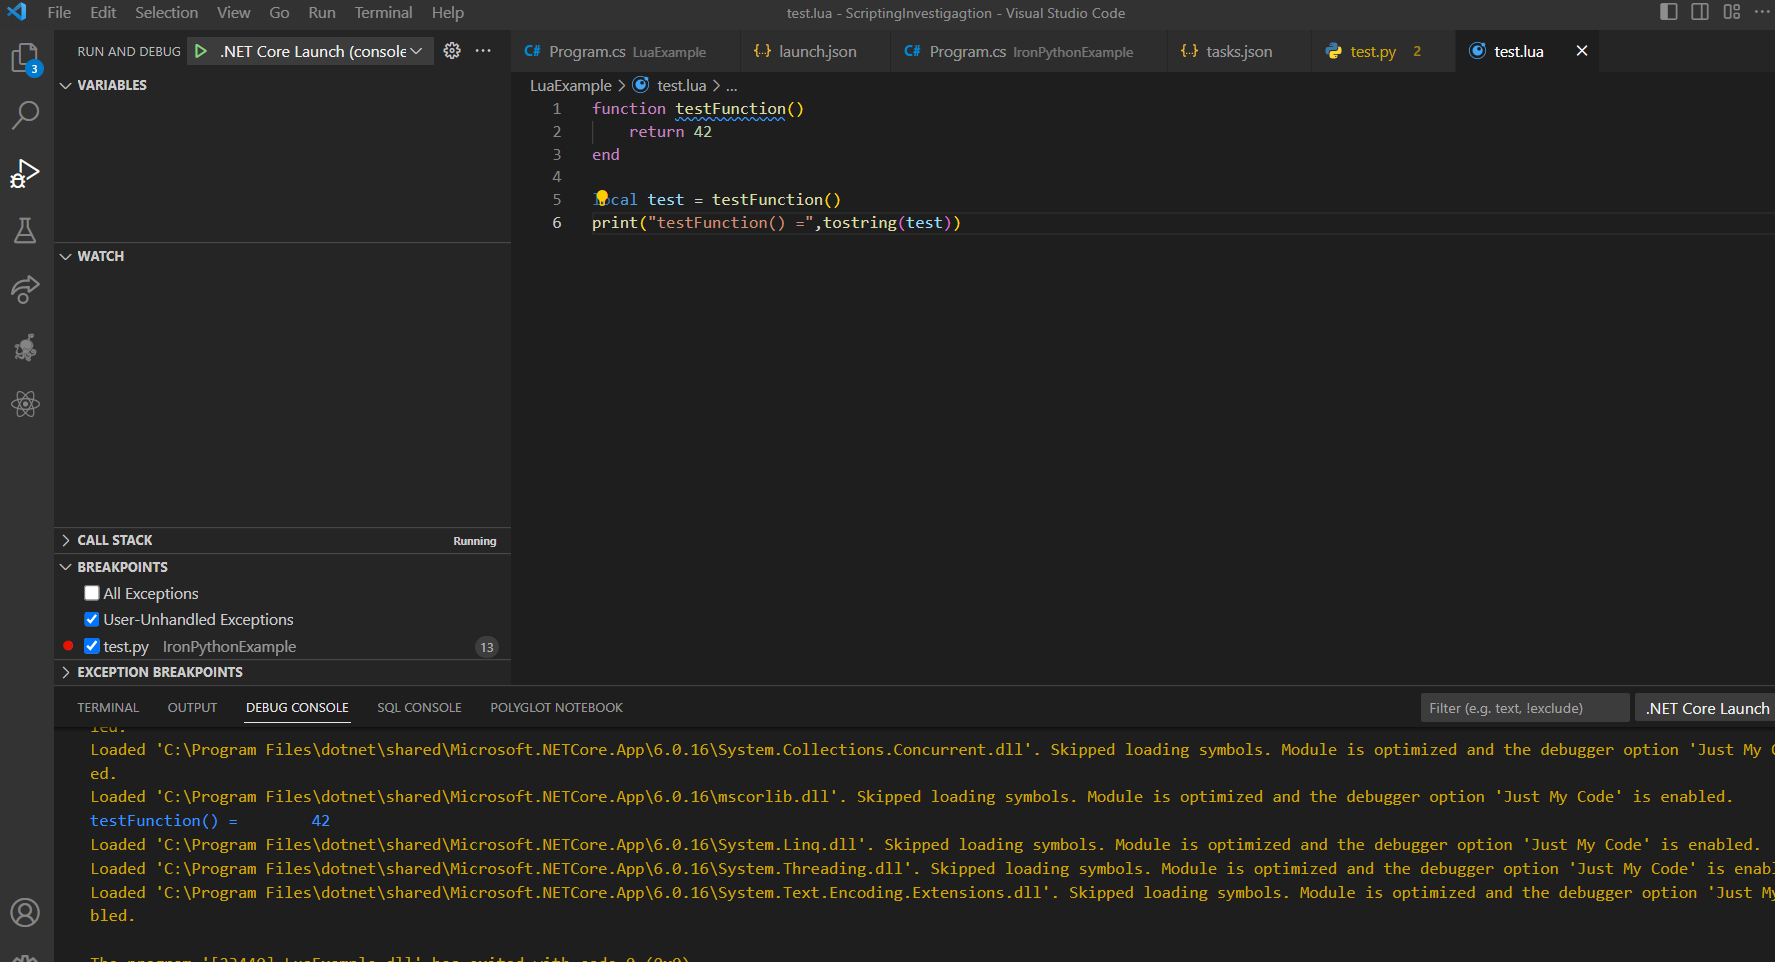
\includegraphics[scale=0.5]{pics/Lua-Konsolenausgabe.png}
        \caption{Lua-Konsolenausgabe}
        \label{fig:impl:KonsolenausgabeLua}
    \end{figure}

\newpage
    \item Die Beweise für das Debugging mit IronPython:
    \begin{figure}[H]
        \centering
        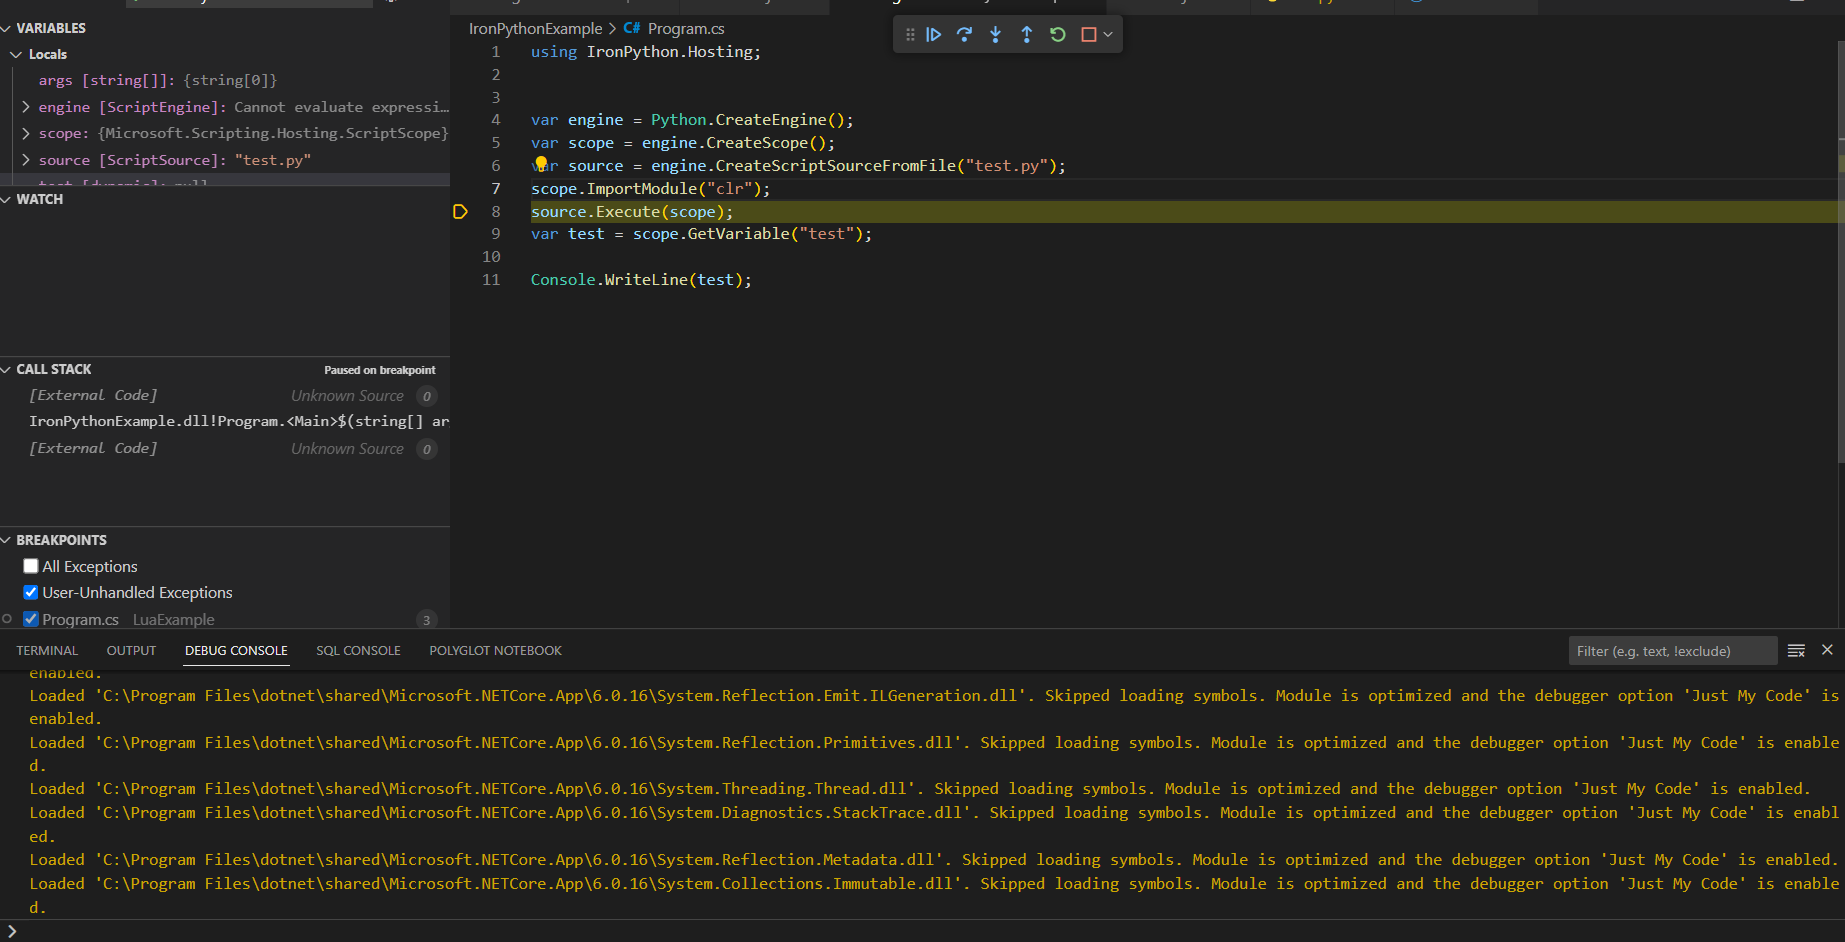
\includegraphics[scale=0.5]{pics/IronPythonVSCodeBreakpoint1.png}
        \caption{IronPython-VSCode-Breakpoint1}
        \label{fig:impl:IronPythonVSCodeBreakpoint1}
    \end{figure}

    \begin{figure}[H]
        \centering
        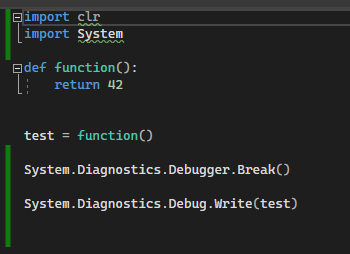
\includegraphics{pics/IronPythonVSBreakpoint2.png}
        \caption{IronPython-VSBreakpoint2}
        \label{fig:impl:IronPythonVSBreakpoint2}
    \end{figure}

    \begin{figure}[H]
        \centering
        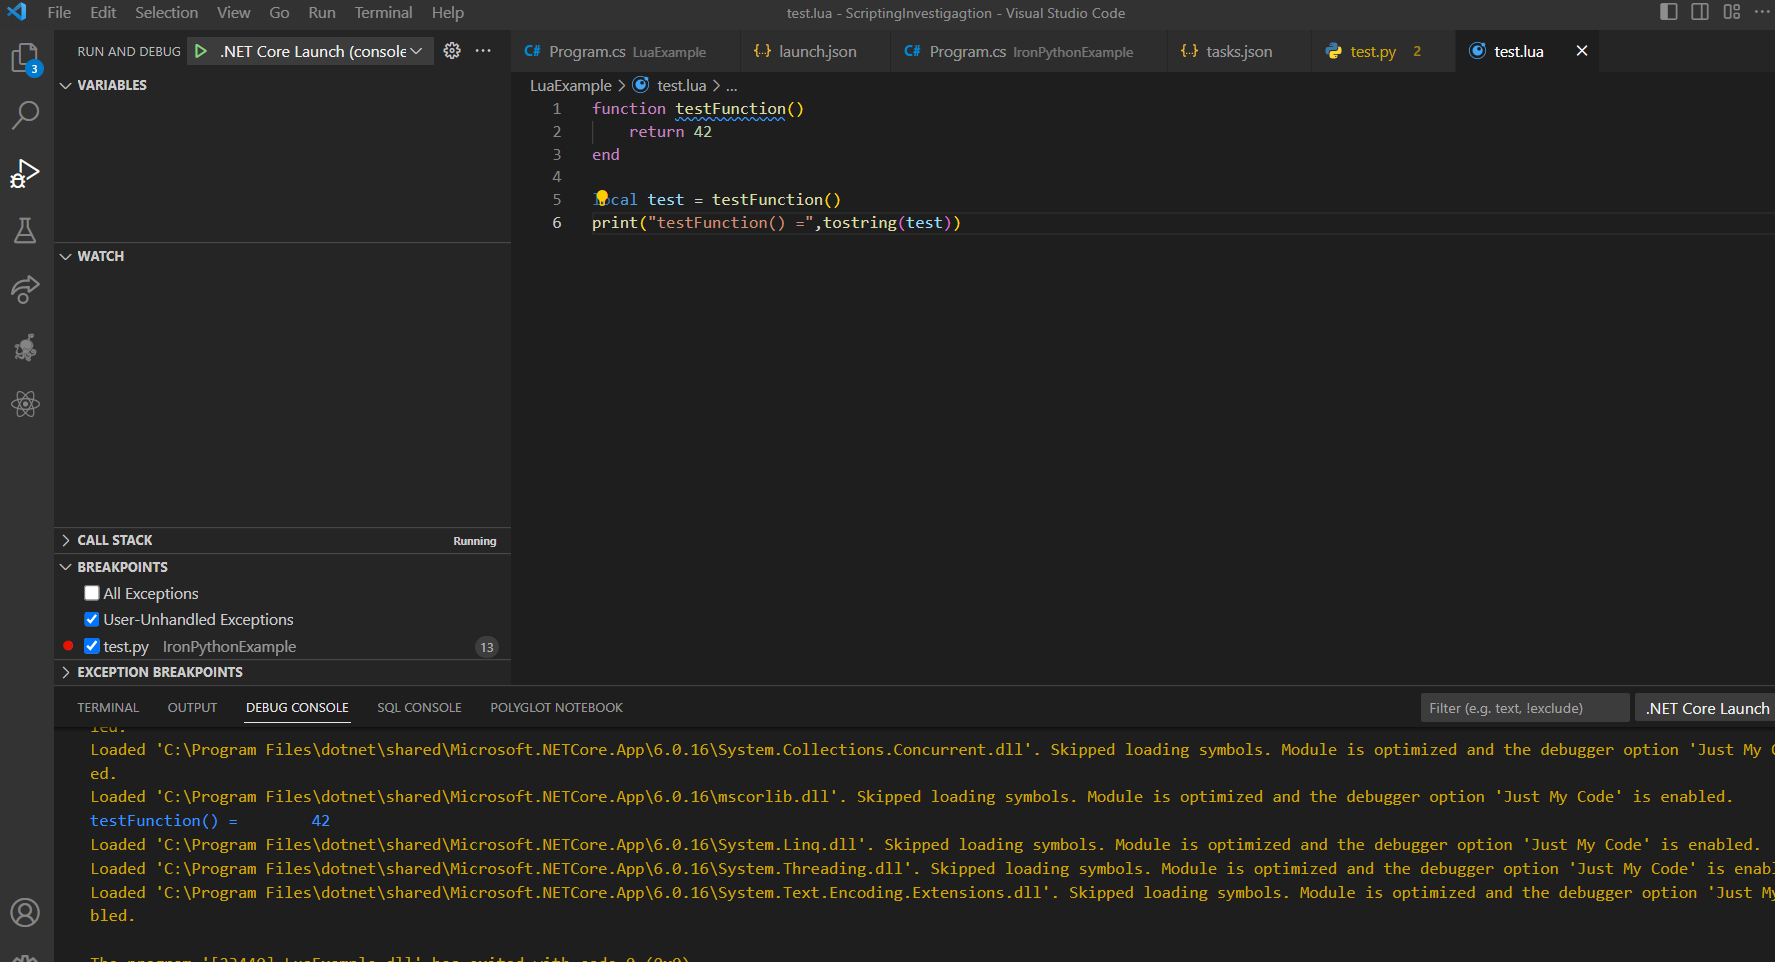
\includegraphics[scale=0.5]{pics/IronPythonKonsolenausgabe.png}
        \caption{IronPython-Konsolenausgabe}
        \label{fig:impl:IronPythonKonsolenausgabe}
    \end{figure}
\end{itemize}